% =============================================================================
% Sec-C PhD Report — TikZ & pgfplots Templates
% Referenced by generate-report skill. Copy relevant diagrams into chapter files.
% =============================================================================
% Required preamble (add to main.tex before first use):
%   \usepackage{tikz}
%   \usepackage{pgfplots}
%   \pgfplotsset{compat=1.18}
%   \usetikzlibrary{shapes.geometric, arrows.meta, positioning, automata, calc, fit, backgrounds}
%   \usepackage{algorithm}
%   \usepackage{algpseudocode}
%   \usepackage{mathtools}
% =============================================================================


%% ============ DIAGRAM 1: Cascade Architecture ============
%% Use in: Ch1 (high-level), Ch3 (detailed version)
\begin{figure}[H]
\centering
\begin{tikzpicture}[
    stage/.style={draw, rounded corners, minimum width=3.5cm, minimum height=1.2cm, align=center, font=\small\bfseries},
    arrow/.style={-{Stealth[length=3mm]}, thick},
    resolved/.style={-{Stealth[length=3mm]}, thick, dashed, color=green!60!black},
    escalated/.style={-{Stealth[length=3mm]}, thick, color=red!60!black},
    label/.style={font=\footnotesize, midway, above},
    pct/.style={font=\footnotesize\itshape, midway, below}
]
    \node[stage, fill=blue!15] (input) {Source Code\\Input};
    \node[stage, fill=orange!20, right=2cm of input] (sast) {Stage 1\\SAST Pre-Screener};
    \node[stage, fill=yellow!20, right=2cm of sast] (graph) {Stage 2\\Graph Validator};
    \node[stage, fill=red!15, below=2cm of graph] (llm) {Stage 3\\LLM Dual-Agent};
    \node[stage, fill=green!15, below=2cm of sast] (fusion) {Stage 4\\Score Fusion};
    \node[stage, fill=purple!15, left=2cm of fusion] (report) {Final\\Report};

    \draw[arrow] (input) -- (sast);
    \draw[resolved] (sast) -- node[label] {Resolved} node[pct] {$\sim$75\%} (fusion);
    \draw[escalated] (sast) -- node[label] {Escalated} node[pct] {$U \geq 0.5$} (graph);
    \draw[resolved] (graph) -- node[label, right] {Singleton} (fusion);
    \draw[escalated] (graph) -- node[label] {Ambiguous} (llm);
    \draw[arrow] (llm) -- node[label, left] {Validated} (fusion);
    \draw[arrow] (fusion) -- (report);
\end{tikzpicture}
\caption{Four-stage cascade architecture with uncertainty-driven escalation. Findings are resolved at the cheapest possible stage; only ambiguous cases are escalated to more expensive analysis.}
\label{fig:cascade_architecture}
\end{figure}


%% ============ DIAGRAM 2: Finding Lifecycle State Machine ============
%% Use in: Ch3 Section 3.6
\begin{figure}[H]
\centering
\begin{tikzpicture}[
    state/.style={draw, circle, minimum size=1.5cm, align=center, font=\scriptsize\bfseries},
    arrow/.style={-{Stealth[length=2.5mm]}, thick},
    every edge/.style={draw, arrow},
    node distance=3cm
]
    \node[state, fill=gray!20] (new) {NEW};
    \node[state, fill=orange!20, right=of new] (sast) {SAST\\Scored};
    \node[state, fill=green!20, above right=1.5cm and 2.5cm of sast] (sast_r) {SAST\\Resolved};
    \node[state, fill=yellow!20, right=of sast] (graph) {Graph\\Validated};
    \node[state, fill=green!20, above right=1.5cm and 2.5cm of graph] (graph_r) {Graph\\Resolved};
    \node[state, fill=red!15, right=of graph] (llm) {LLM\\Validated};
    \node[state, fill=purple!20, below=2cm of graph] (fused) {Score\\Fused};

    \path (new) edge node[above, font=\scriptsize] {pre-screen} (sast);
    \path (sast) edge node[above, font=\scriptsize, sloped] {$U < 0.5$} (sast_r);
    \path (sast) edge node[above, font=\scriptsize] {$U \geq 0.5$} (graph);
    \path (graph) edge node[above, font=\scriptsize, sloped] {singleton} (graph_r);
    \path (graph) edge node[above, font=\scriptsize] {ambiguous} (llm);
    \path (sast_r) edge[bend right=20] (fused);
    \path (graph_r) edge (fused);
    \path (llm) edge[bend left=20] (fused);
\end{tikzpicture}
\caption{Finding lifecycle through the four-stage cascade. Each finding enters as NEW and exits with a fused score after resolution at the earliest possible stage.}
\label{fig:finding_lifecycle}
\end{figure}


%% ============ DIAGRAM 3: Mini-GAT Architecture ============
%% Use in: Ch3 Section 3.3.4
\begin{figure}[H]
\centering
\begin{tikzpicture}[
    layer/.style={draw, rounded corners, minimum width=2.5cm, minimum height=0.8cm, align=center, font=\small},
    arrow/.style={-{Stealth[length=2.5mm]}, thick},
    dim/.style={font=\scriptsize\itshape, text=gray}
]
    \node[layer, fill=blue!10] (input) {Input Features};
    \node[dim, right=0.3cm of input] {$\mathbb{R}^{N \times 773}$};

    \node[layer, fill=orange!15, below=1cm of input] (gat1) {GATConv Layer 1\\(4 heads, ELU, dropout)};
    \node[dim, right=0.3cm of gat1] {$\mathbb{R}^{N \times 1024}$};

    \node[layer, fill=yellow!15, below=1cm of gat1] (gat2) {GATConv Layer 2\\(4 heads, concat=False)};
    \node[dim, right=0.3cm of gat2] {$\mathbb{R}^{N \times 128}$};

    \node[layer, fill=green!15, below=1cm of gat2] (pool) {Global Mean Pooling};
    \node[dim, right=0.3cm of pool] {$\mathbb{R}^{128}$};

    \node[layer, fill=red!10, below left=1cm and -0.5cm of pool] (cls) {Classification Head\\Linear(128, 2) + Softmax};
    \node[layer, fill=purple!10, below right=1cm and -0.5cm of pool] (conf) {Confidence Head\\Linear(128, 1) + Sigmoid};

    \draw[arrow] (input) -- (gat1);
    \draw[arrow] (gat1) -- (gat2);
    \draw[arrow] (gat2) -- (pool);
    \draw[arrow] (pool) -| (cls);
    \draw[arrow] (pool) -| (conf);
\end{tikzpicture}
\caption{Mini-GAT architecture. Input combines 768-dimensional GraphCodeBERT embeddings with 5 structural features. Two GAT layers with multi-head attention produce graph-level representations for vulnerability classification and confidence estimation.}
\label{fig:mini_gat}
\end{figure}


%% ============ DIAGRAM 4: Training Curves Template (pgfplots) ============
%% Use in: Ch4 Section 4.2
%% Replace coordinate values with actual data from notebook outputs
\begin{figure}[H]
\centering
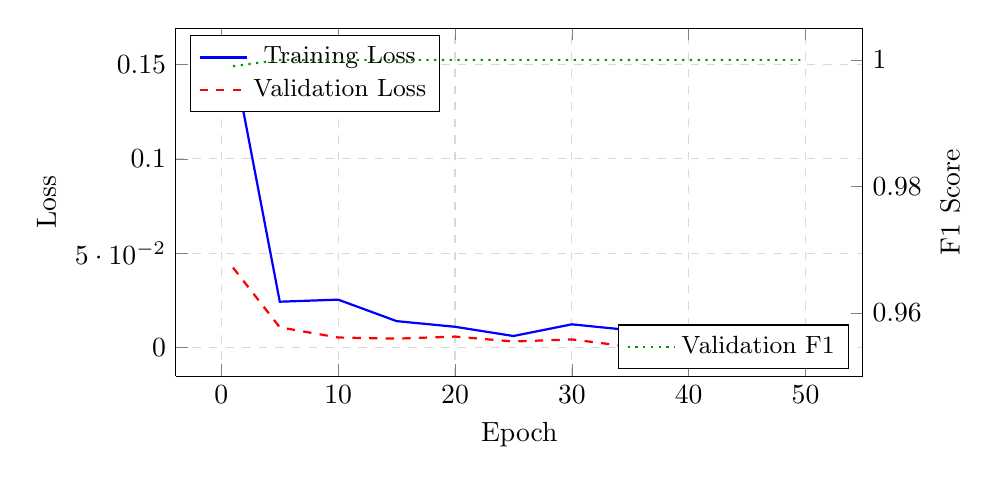
\begin{tikzpicture}
\begin{axis}[
    width=0.85\linewidth,
    height=6cm,
    xlabel={Epoch},
    ylabel={Loss},
    axis y line*=left,
    legend style={at={(0.02,0.98)}, anchor=north west, font=\small},
    grid=major,
    grid style={dashed, gray!30},
]
    % %%% DATA %%% Replace with actual epoch-loss values from notebook outputs
    \addplot[blue, thick, mark=none] coordinates {
        (1,0.1539) (5,0.0242) (10,0.0253) (15,0.0139) (20,0.0109)
        (25,0.0060) (30,0.0122) (35,0.0091) (40,0.0079) (45,0.0063) (50,0.0081)
    };
    \addlegendentry{Training Loss}
    \addplot[red, thick, dashed, mark=none] coordinates {
        (1,0.0423) (5,0.0106) (10,0.0052) (15,0.0046) (20,0.0057)
        (25,0.0031) (30,0.0042) (35,0.0003) (40,0.0033) (45,0.0001) (50,0.0055)
    };
    \addlegendentry{Validation Loss}
\end{axis}
\begin{axis}[
    width=0.85\linewidth,
    height=6cm,
    ylabel={F1 Score},
    axis y line*=right,
    axis x line=none,
    legend style={at={(0.98,0.02)}, anchor=south east, font=\small},
    ymin=0.95, ymax=1.005,
]
    \addplot[green!60!black, thick, dotted, mark=none] coordinates {
        (1,0.999) (5,1.000) (10,1.000) (15,1.000) (20,1.000)
        (25,1.000) (30,1.000) (35,1.000) (40,1.000) (45,1.000) (50,1.000)
    };
    \addlegendentry{Validation F1}
\end{axis}
\end{tikzpicture}
\caption{GNN V1 training curves on the Juliet Test Suite (54,147 samples). %%% UPDATE CAPTION %%%}
\label{fig:training_curves_v1}
\end{figure}


%% ============ DIAGRAM 5: Confusion Matrix ============
%% Use in: Ch4 Section 4.2
%% Replace %%% N %%% with actual values from notebook outputs
\begin{figure}[H]
\centering
\begin{tikzpicture}[
    cell/.style={minimum width=2.5cm, minimum height=2.5cm, align=center, font=\large\bfseries}
]
    \node at (1.25, 3.5) {\textbf{Predicted}};
    \node[rotate=90] at (-1.5, 1.25) {\textbf{Actual}};
    \node at (0, 3) {\small Safe};
    \node at (2.5, 3) {\small Vulnerable};
    \node at (-1, 2.5) {\small Safe};
    \node at (-1, 0) {\small Vulnerable};

    % %%% DATA %%% Replace with actual values
    \node[cell, fill=green!30] at (0, 2.5) {TN\\%%% N %%%};
    \node[cell, fill=red!20] at (2.5, 2.5) {FP\\%%% N %%%};
    \node[cell, fill=red!20] at (0, 0) {FN\\%%% N %%%};
    \node[cell, fill=green!30] at (2.5, 0) {TP\\%%% N %%%};
\end{tikzpicture}
\caption{Confusion matrix for GNN V1/V2 on the test set. %%% UPDATE %%%}
\label{fig:confusion_matrix}
\end{figure}


%% ============ DIAGRAM 6: Cascade Funnel ============
%% Use in: Ch4 Section 4.4
%% Replace %%% N %%% with actual cascade statistics
\begin{figure}[H]
\centering
\begin{tikzpicture}[
    box/.style={draw, rounded corners, minimum height=1cm, align=center, font=\small\bfseries},
    arrow/.style={-{Stealth[length=2.5mm]}, thick}
]
    \node[box, fill=blue!15, minimum width=12cm] (all) {All Findings: %%% N %%%};
    \node[box, fill=orange!15, minimum width=9cm, below=0.8cm of all] (sast) {After SAST: %%% N %%% escalated};
    \node[box, fill=yellow!15, minimum width=6cm, below=0.8cm of sast] (graph) {After Graph: %%% N %%% escalated};
    \node[box, fill=red!15, minimum width=3cm, below=0.8cm of graph] (llm) {After LLM: %%% N %%% confirmed};

    \draw[arrow] (all) -- (sast) node[midway, right, font=\scriptsize] {%%% \% resolved %%%};
    \draw[arrow] (sast) -- (graph) node[midway, right, font=\scriptsize] {%%% \% resolved %%%};
    \draw[arrow] (graph) -- (llm) node[midway, right, font=\scriptsize] {%%% \% resolved %%%};
\end{tikzpicture}
\caption{Cascade funnel showing progressive finding reduction through each stage.}
\label{fig:cascade_funnel}
\end{figure}


%% ============ DIAGRAM 7: Baseline Comparison Bar Chart ============
%% Use in: Ch4 Section 4.8
%% Replace coordinate values with actual comparison metrics
\begin{figure}[H]
\centering
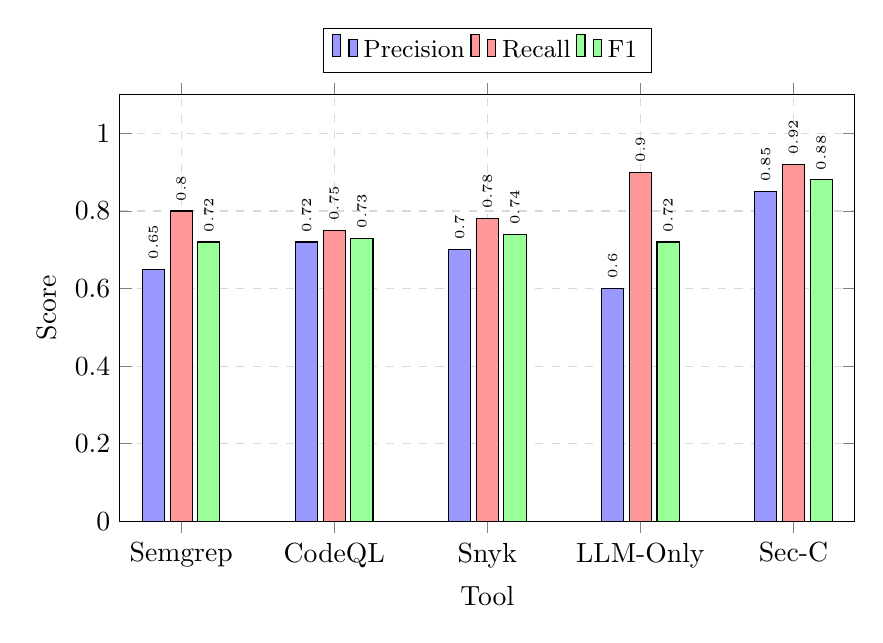
\begin{tikzpicture}
\begin{axis}[
    width=0.9\linewidth,
    height=7cm,
    ybar=2pt,
    bar width=8pt,
    xlabel={Tool},
    ylabel={Score},
    ymin=0, ymax=1.1,
    symbolic x coords={Semgrep, CodeQL, Snyk, LLM-Only, Sec-C},
    xtick=data,
    legend style={at={(0.5,1.05)}, anchor=south, legend columns=4, font=\small},
    grid=major,
    grid style={dashed, gray!30},
    nodes near coords,
    every node near coord/.append style={font=\tiny, rotate=90, anchor=west},
]
    % %%% DATA %%% Replace with actual comparison values
    \addplot[fill=blue!40] coordinates {(Semgrep,0.65) (CodeQL,0.72) (Snyk,0.70) (LLM-Only,0.60) (Sec-C,0.85)};
    \addplot[fill=red!40] coordinates {(Semgrep,0.80) (CodeQL,0.75) (Snyk,0.78) (LLM-Only,0.90) (Sec-C,0.92)};
    \addplot[fill=green!40] coordinates {(Semgrep,0.72) (CodeQL,0.73) (Snyk,0.74) (LLM-Only,0.72) (Sec-C,0.88)};
    \legend{Precision, Recall, F1}
\end{axis}
\end{tikzpicture}
\caption{Comparative performance of Sec-C against baseline tools. %%% UPDATE with actual metrics %%%}
\label{fig:baseline_comparison}
\end{figure}


%% ============ DIAGRAM 8: Dual-Agent Interaction ============
%% Use in: Ch3 Section 3.4
\begin{figure}[H]
\centering
\begin{tikzpicture}[
    agent/.style={draw, rounded corners, minimum width=3cm, minimum height=1.5cm, align=center, font=\small\bfseries},
    arrow/.style={-{Stealth[length=2.5mm]}, thick},
    data/.style={draw, dashed, rounded corners, minimum width=2.5cm, minimum height=0.8cm, align=center, font=\scriptsize}
]
    \node[data, fill=gray!10] (finding) {Finding + Code Context\\+ RAG Knowledge};

    \node[agent, fill=red!15, below left=2cm and 1cm of finding] (attacker) {Attacker Agent\\(Red Team)};
    \node[agent, fill=blue!15, below right=2cm and 1cm of finding] (defender) {Defender Agent\\(Blue Team)};

    \node[data, fill=red!10, below=1.5cm of attacker] (av) {AttackerVerdict\\confidence, reasoning,\\CVSS sub-metrics};
    \node[data, fill=blue!10, below=1.5cm of defender] (dv) {DefenderVerdict\\confidence, reasoning,\\sanitizer analysis};

    \node[agent, fill=purple!15, below=1cm of finding, yshift=-7cm] (consensus) {Consensus Engine\\(4 Rules)};

    \node[data, fill=green!10, below=1.5cm of consensus] (output) {LLMValidation\\verdict, fused\_confidence,\\CVSS score, evidence};

    \draw[arrow] (finding) -| (attacker);
    \draw[arrow] (finding) -| (defender);
    \draw[arrow] (attacker) -- (av);
    \draw[arrow] (defender) -- (dv);
    \draw[arrow] (av) |- (consensus);
    \draw[arrow] (dv) |- (consensus);
    \draw[arrow] (consensus) -- (output);
\end{tikzpicture}
\caption{Dual-agent adversarial validation protocol. The attacker agent analyzes exploitability while the defender agent identifies sanitizers. A consensus engine combines both verdicts using four decision rules.}
\label{fig:dual_agent}
\end{figure}
